% Ideia básica dos algorítmos (Coesão léxica ) como **presuposto básico**

Os principais algoritmos de segmentação textual baseiam-se na ideia de coesão léxica entre assuntos. Isto é, a mudança de tópicos é acompanhada de uma proporcional mudança de vocabulário. A partir disso, vários algoritmos foram propostos. Dessa forma, assumem o pressuposto que um segmento pode ser identificado e delimitado pela análise das palavras que o compõe.







% A coesão léxica é um termômetro para as mudanças de tópicos, e portanto, um indicador para quebras de segmento.

 
 
% Nesse artigo, os principais serão analisados na perspectiva de atas de reunião.


%Os principais algoritmos de segmentação textual assumem o pressuposto que um segmento pode ser identificado e delimitado pela análise de seu vocabulário





%Os entre os principais trabalhos relacionados a segmentação textual estão o \textit{TextTiling} e o \textit{C99}



%\subsubsection{TextTiling}
%	O algoritmo TextTiling, proposto por 
	
%
%\subsubsection{C99}



Entre os mais influentes podemos citar o \textit{TextTiling}~\cite{Hearst1994} 




Semelhante a esse trabalho, outras abordagens foram propostas como ...

\cite{Banerjee200657} faz uma adaptação do \textit{TextTiling} ao contexto das conversas em reuniões com múltiplos participantes.  



%%%%%%%
% C99 %
%%%%%%%

Choi \cite{Choi2000} apresenta um trabalho que usa \textit{cosine}, a qual é exibida na equação~\ref{equ:cosine}, como medida similaridade e apresenta um esquema de ranking em seu algoritmo, o C99. 
%
Embora muitos dos melhores trabalho utilizarem matrizes de similaridades, o autor traz obervações.
%
Ele aponta que para pequenos segmentos, o cálculo de suas similaridades não é confiável. Pois uma ocorrência adicional de uma palavra causa um impacto desproporcional no cálculo.
%
Além disso, o estilo da escrita pode não ser constante em todo o texto. Choi sugere que, por exemplo, textos iniciais dedicados a introdução costumam apresentar menor coesão do que trechos dedicados a um tópico específico. 
%

Portanto comparar a similaridade entre trechos de diferentes regiões, não é apropriado.
% Complexidade O(n²)
Devido a isso, as similaridades não podem ser comparadas em valores absolutos,  então, o autor apresenta um esquema de ranking para contornar esse problema.
%

Cada valor na matriz de similaridade é substituído por seu ranking local. Onde ranking é o número de elementos vizinhos com similaridade menor, o qual e calculado com a equação~\ref{equ:ranklocal}. Um exemplo é mostrado na Figura \ref{fig:exemplomatrixrank} abaixo.



  \begin{figure}[!h]

	\centering
	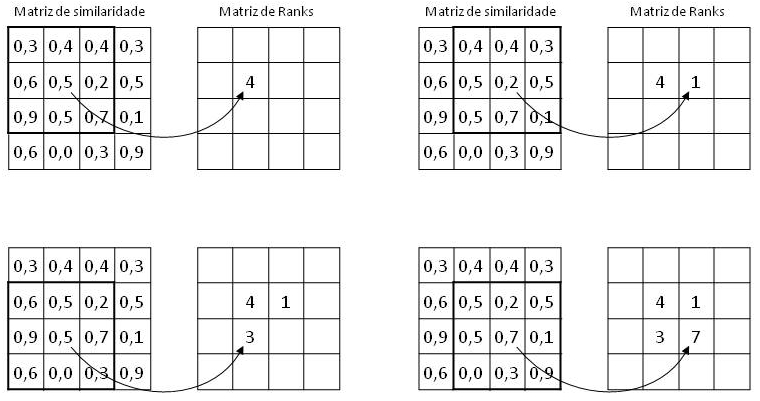
\includegraphics[width=0.45\textwidth]{exemplo-matrix-rank-noborder.jpg}
	\caption{Exemplo de construção de uma matriz de rank}
	\label{fig:exemplomatrixrank}

  \end{figure}


  \begin{figure}[!h]

	\centering
	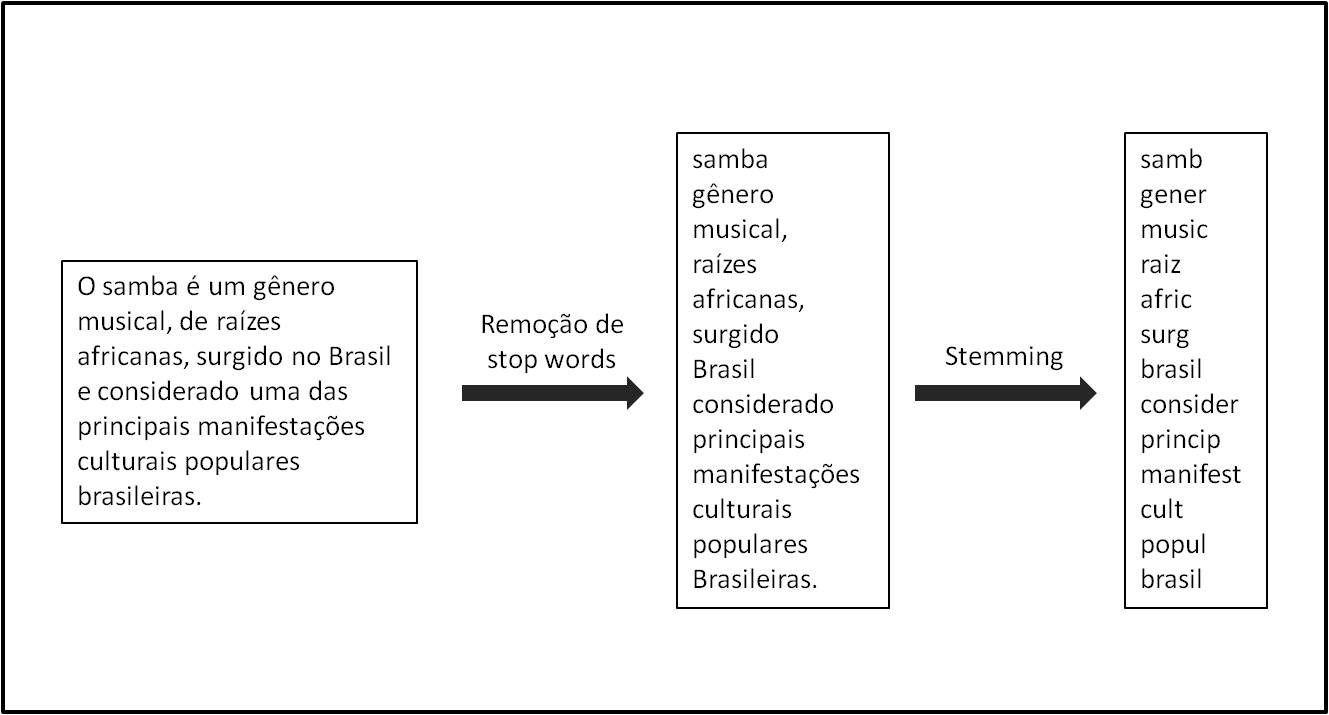
\includegraphics[width=0.45\textwidth]{exemplo-preprocessamento.jpg}
	\caption{Exemplo de preprocessamento}
	\label{fig:exemplomatrixrank}

  \end{figure}




\begin{equation}
Sim(x,y) = \frac
{\Sigma_j f_{x,j} \times f_{y,j}}
{\sqrt{\Sigma_j f^2_{x,j} \times \Sigma f^2_{x,j}}}
\label{equ:cosine}
\end{equation}



\begin{equation}
r(x,y) = \frac
{Numero\ de\ elementos\ com\ similaridade\ menor}
{Numero\ de\ elementos\ examinados}
\label{equ:ranklocal}
\end{equation}












